\documentclass[12pt]{article}

\usepackage{baseset}
\DeclareSymbolFont{operators}{OT1}{ntxtlf}{m}{n}
\SetSymbolFont{operators}{bold}{OT1}{ntxtlf}{b}{n}
\newcommand{\RomanNumeralCaps}[1]
{\MakeUppercase{\romannumeral #1}}
\usepackage{enumitem}

\begin{document}
	\section*{1.4.1 Изучение физического маятника}
	\textit{Выполнила Красоткина Виктория, Б01-203}
	
	\textbf{Цель:} исследовать зависимость периода колебаний физического маятника от его момента инерции, проверить справедливость формулы для периода колебаний физического маятника и определить значение ускорения свободного падения и убедиться в справедливости теоремы Гюйгенса об обратимости	точек опоры и центра качания маятника.
	
	\textbf{Приборы:}
	
	\begin{itemize}
		\item физический маятник (однородный стальной стержень)
		\item опорная призма
		\item математический маятник
		\item счетчик числа колебаний
		\item линейка
		\item секундомер
	\end{itemize}

	\subsection*{Теоретическая часть}
	\begin{wrapfigure}{l}{6cm}
		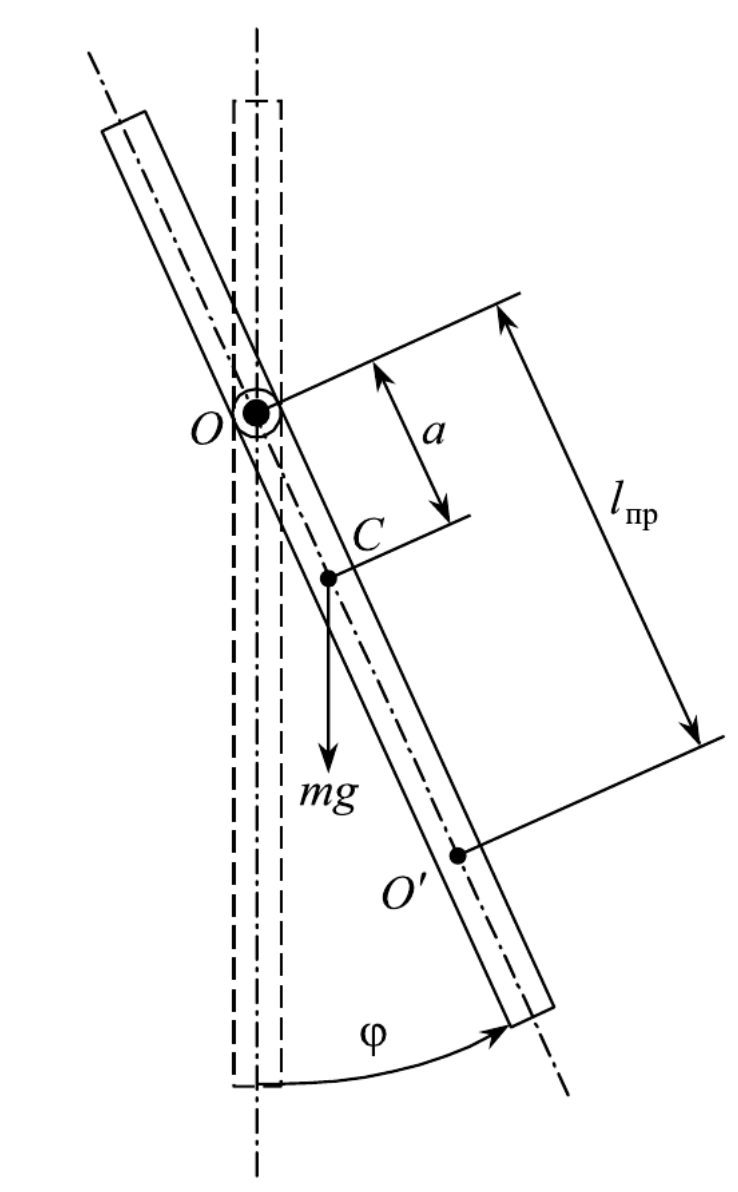
\includegraphics[width=\linewidth]{physm_pic}
		\captionof{figure}{Физический маятник}
		\label{physm_pic}	
	\end{wrapfigure}
	
	\textit{Физический маятник} --- любое твердое тело, которое под действием силы тяжести может свободно качаться вокруг неподвижной горизонтальной оси. Движение маятника описывается уравнением
	\begin{equation}\label{eq1}
		I\frac{d^2\phi}{dt^2}=M,
	\end{equation}
	где $I$ --- момент инерции маятника, $\phi$ --- угол отклонения маятника от пложения равновесия, $t$ --- время, $M$ --- момент сил, действующих на маятник.
	
	В работе используется однородный стальной стержень длиной $l$, на котором закреплена опорная призма, ее острое ребро является осью качания маятника. Расстояние $OC = a$ (см. рис. \ref{physm_pic}) --- расстояние от точки опоры до центра масс. которое можно менять передвижением призмы. Подвесная призма остаётся неподвижной ($a = const$), а на стержень маятника насаживается дополнительное тело небольшого размера, положение которого можно изменять, изменяя таким образом момент инерции маятника. Период колебаний маятника в этой схеме измеряется электронным счетчиком импульсов, расположенном у нижнего конца стержня.
	
	По теореме Гюйгенса-Штейнера момент инерции маятника
	$$
	I = \frac{ml^2}{12} + ma^2,
	$$
	где $m$ --- масса маятника. Момент силы, действующей на маятник:
	$$
	M = -mga\sin{\varphi}\approx-mga\varphi
	$$
	Приближенное равенство работает при малых значениях угла.
	
	Подставляя выражения для моментов инерции и сил в уравнение (\ref{eq1}), получаем уравнение колебаний:
	$$
	\ddot{\varphi} + \omega^2\varphi = 0,
	$$
	где
	$$
	\omega^2 = \frac{ga}{a^2 + \dfrac{l^2}{12}}
	$$
	Решение уравнения колебаний:
	$$
	\varphi(t) = A\sin{(\omega t + \alpha)},
	$$
	где $A$ --- амплитуда колебаний, $\alpha$ --- начальная фаза маятника.
	
	Период колебаний физического маятника: 
	\begin{equation}\label{period_eq}
	T = \frac{2\pi}{\omega} = 2\pi\sqrt{\frac{a^2+\dfrac{l^2}{12}}{ag}}
	\end{equation}
	Период колебаний математического маятника:
	$$
	T' = 2\pi\sqrt{\frac{l'}{g}},
	$$
	где $l'$ --- длина математического маятника. Величину $a^2+\dfrac{l^2}{12} = l_{\text{пр}}$ называют приведенной длиной физического маятника.
	
	В качестве подвижного груза в работе используется металлический цилиндр или «чечевица». Поскольку размер груза мал по сравнению с длиной стержня, его можно считать закреплённой на стержне точечной массой. Обозначим за $y$ расстояние от точки подвеса $O$ до центра масс груза (см. рис. \ref{inertion}). Тогда момент инерции маятника будет равен
	$$
	I = I_0 + m_{\text{г}}y^2
	$$
	\begin{wrapfigure}{l}{3cm}
		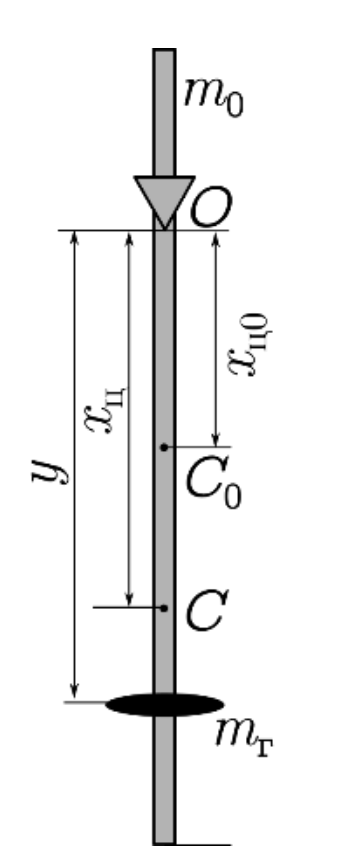
\includegraphics[width=\linewidth]{inertion}
		\caption{Маятник с дополнительным грузом}
		\label{inertion}	
	\end{wrapfigure}
	Пусть $x_{\text{ц0}}$ --- расстояние от точки подвеса (острия	призмы) до центра масс маятника без груза. Тогда центр масс маятника с грузом находится в точке
	\begin{equation}\label{x_eq}
	x_{\text{ц}} = \frac{m_0x_{\text{ц0}} + m_{\text{г}}y}{M},
	\end{equation}
	где $m_0$ --- масса маятника без груза (стержня вместе с призмой), $M = m_0 + m_{\text{г}}$ --- полная масса маятника. Положения центра масс $	x_{\text{ц}}$ и $x_{\text{ц0}}$ могут быть измерены с
	помощью подставки. Отсюда находим формулу для вычисления положения центра масс груза:
	$$
	y = \frac{Mx_{\text{ц}} - m_0x_{\text{ц0}}}{m_{\text{г}}}
	$$
	Период колебаний маятника:
	\begin{equation}\label{T_eq}
	T = 2\pi\sqrt{\frac{I_0 + m_{\text{г}}y^2}{gMx_{\text{ц}}}}
	\end{equation}
	Отсюда видно, что если построить зависимость величины $u = T^2x_{\text{ц}}$ от $v = y^2$, то график должен иметь вид прямой линии. По её наклону можно определить ускорение свободного падения $g$, а по вертикальному смещению --- момент инерции $I_0$ маятника.
	\subsection*{Ход работы}
	\begin{enumerate}[label={\textbf{\arabic*.}}]
		\item Погрешность
		\begin{itemize}
			\item линейки --- $1$ мм
			\item штангенциркуля --- $0.1$ мм
			\item секундомера --- $0.03$ с
			\item весов --- $0.1$ г
		\end{itemize}
		\item Запишем измеренные данные о стержне, призме и грузе:
		\begin{itemize}
			\item Длина стержня $l = 100.1\pm0.1$ см
			\item Масса призмы $m_{\text{п}} = 75.6\pm0.1~\text{г}$
			\item Масса стержня $m = 944.0\pm0.1~\text{г}$
			\item Масса груза $m_{\text{г}} = 312.6\pm0.1~\text{г}$
		\end{itemize}
		\item Центра масс призмы расположен на расстоянии $50.1\pm0.1$ см. Положение призмы (расстояние между остриём призмы и центром масс стержня): 
		$$
		a = 30.3\pm0.1~\text{см}
		$$
		Положение центра масс конструкции (расстояние между остриём призмы и центром масс конструкции): $$
		x_\text{ц} = 28.1\pm0.1~\text{см}
		$$
		Кроме цены деления на погрешность определения величин влияет то, что достичь точного равновесия очень сложно.
		\item Проведем первый предварительный опыт по измерению периода колебаний без дополнительного груза: измерим время $20$ колебаний и найдем период. Получим $T = 1.529$ с. При таком значении периода $g = 9.75~\frac{\text{м}}{\text{с}^2}$.
		После этого проведем серию измерений для экспериментального определения случайной погрешности измерения времени с помощью секундомера. Запишем в таблицу \ref{null_ex} данные, полученные в этом опыте.
		\begin{table}[h]
			\centering
			\begin{tabular}{|c|c|c|}\hline
				№   & $t$, с  & $T$, с \\ \hline
				$1$ & $30.58$ &	$1.529$ \\
				$2$	& $30.59$ &	$1.5295$ \\
				$3$ & $30.57$ &	$1.5285$ \\
				$4$ & $30.57$ &	$1.5285$ \\
				$5$ & $30.59$ &	$1.5295$ \\
				$6$ & $30.58$ &	$1.529$  \\
				$7$ & $30.57$ &	$1.5285$ \\
				$8$ & $30.57$ &	$1.5285$ \\ \hline	
			\end{tabular}
			\caption{предварительный опыт}
			\label{null_ex}
		\end{table}
		Рассчитаем среднее значение периода:
		$$
		T = 1.53~\text{с}
		$$
		Рассчитаем погрешность полученного результата:
		$$
		\sigma_{\text{пр}} = 0.03~\text{с},~\sigma_{\text{сл}} = \sqrt{\frac{1}{n-1}\sum_{i=1}^n \left(T_i - \overline{T}\right)^2} = 4.6\cdot10^{-4} \approx 0~\text{с},~\sigma_T = \sqrt{\sigma_{\text{пр}}^2 + \sigma_{\text{сл}}^2} = 0.03~\text{с}
		$$
		Тогда
		$$
		T = 1.53\pm0.03~\text{с},~\varepsilon = 2\%
		$$
		Теперь по формуле (\ref{period_eq}) рассчитаем значение $g$:
		$$
		g = \frac{4\pi^2}{T^2}\cdot\frac{x_\text{ц}^2+\dfrac{l^2}{12}}{x_\text{ц}} = 9.75~\frac{\text{м}}{\text{с}^2}
		$$
		Погрешность рассчитаем следующим образом:
		$$
		\sigma_g = g\cdot\sqrt{\left(\frac{\partial g}{\partial x_\text{ц}}\right)^2 + \left(\frac{\partial g}{\partial l}\right)^2 + \left(\frac{\partial g}{\partial T}\right)^2} \approx 0.38,~\varepsilon = 4\%
		$$
		Полученное значение попадает в ворота точности $10\%$.
		\item Чтобы погрешность измерений соответствовала точности измерений $\varepsilon_{max} = 0.1\%$, необходимое число колебаний, по которому следует измерять период, равно
		$$
		n = \frac{0.03\cdot100}{0.1} \cdot\frac{1}{T} \approx 20
		$$
		\item Проведем измерение периода колебаний маятника по $20$ полным колебаниям $10$ раз. Для каждого опыта будем менять значение $y$ --- положение центра масс груза и расчитывать по формуле (\ref{x_eq}) $x_{\text{ц}}$ --- положение центра масс стержня с грузом. Все результаты запишем в таблицу \ref{ex}.
		\begin{table}[h]
			\centering
			\begin{tabular}{|c|c|c|c|c|c|c|c|c|c|}\hline
				№  & $y$,  мм & $x_{\text{ц}}$, мм & $n$ & $t_n$, с & $T$, с & $g$, м/с$^2$ & $\sigma_{\text{пр}}$, м/с$^2$ & $T^2x_{\text{ц}}$, c$^2\cdot$м & $y^2$, м$^2$ \\ \hline
				$1$	 & $650.0$ & $372.8$ & $20$ & $31.45$ & $1.5725$ & $9.68$ & $0.48$ & $0.92$ & $0.4225$ \\
				$2$	 & $600.0$ & $360.4$ & $20$ & $30.87$ & $1.5435$ & $9.68$ & $0.48$ & $0.86$ & $0.3600$ \\
				$3$	 & $550.0$ & $347.9$ & $20$ & $30.34$ & $1.5170$ & $9.67$ & $0.48$ & $0.80$ & $0.3025$ \\
				$4$	 & $500.0$ & $335.5$ & $20$ & $29.87$ & $1.4935$ & $9.66$ & $0.48$ & $0.75$ & $0.2500$ \\
				$5$	 & $450.0$ & $323.0$ & $20$ & $29.42$ & $1.4710$ & $9.68$ & $0.48$ & $0.70$ & $0.2025$ \\
				$6$	 & $400.0$ & $310.6$ & $20$ & $29.06$ & $1.4530$ & $9.68$ & $0.48$ & $0.66$ & $0.1600$ \\
				$7$	 & $350.0$ & $298.2$ & $20$ & $28.80$ & $1.4400$ & $9.67$ & $0.48$ & $0.62$ & $0.1225$ \\
				$8$	 & $300.0$ & $285.7$ & $20$ & $28.60$ & $1.4300$ & $9.69$ & $0.48$ & $0.58$ & $0.0900$ \\
				$9$	 & $250.0$ & $273.3$ & $20$ & $28.54$ & $1.4270$ & $9.68$ & $0.48$ & $0.56$ & $0.0625$ \\
				$10$ & $200.0$ & $260.8$ & $20$ & $28.60$ & $1.4300$ & $9.69$ & $0.48$ & $0.53$ & $0.0400$ \\ \hline
			\end{tabular}
			\caption{основной опыт}
			\label{ex}
		\end{table}
	
		Для каждого измерения рассчитаем значение $g$ из формулы (\ref{T_eq}) и усредним.
		$$
		g = \frac{4\pi^2}{T^2}\cdot\frac{I_0 + m_{\text{г}}y^2}{Mx_{\text{ц}}}
		$$
		Момент инерции $I_0$ (здесь масса стержня рассчитывается с вычетом массы призмы):
		$$
		I_0 = \frac{ml^2}{12} + ma^2 = 0.152\pm0.007~\text{кг$\cdot$м$^2$}
		$$
		Усредним полученные значения $g$ и рассчитаем погрешность.
		$$
		g = 9.68~\frac{\text{м}}{\text{с}^2}
		$$
		$$
		\sigma_{\text{сл}} = \sqrt{\frac{1}{n-1}\sum_{i=1}^n \left(g_i - \overline{g}\right)^2} = 0.01~\frac{\text{м}}{\text{с}^2}
		$$
		$$
		\sigma_{пр} = g\cdot\sqrt{\left(\frac{\partial g}{\partial m_\text{г}}\right)^2 + \left(\frac{\partial g}{\partial M}\right)^2 + \left(\frac{\partial g}{\partial I_0}\right)^2 + \left(\frac{\partial g}{\partial y}\right)^2 + \left(\frac{\partial g}{\partial x_\text{ц}}\right)^2 + \left(\frac{\partial g}{\partial T}\right)^2}
		$$
		Приборную погрешность рассчитываем для каждого измерения и усредняем.
		$$
		\sigma_{пр} = 0.48~\frac{\text{м}}{\text{с}^2}
		$$
		Находим полную погрешность:
		$$
		\sigma = \sqrt{\sigma_{\text{пр}}^2 + \sigma_{\text{сл}}^2} = 0.48~\frac{\text{м}}{\text{с}^2}
		$$
		Тогда
		$$
		g = 9.68\pm0.48~\frac{\text{м}}{\text{с}^2},~\varepsilon = 5\%
		$$
		\item Построим график зависимости $T(y)$.
		\begin{figure}[h]
			\centering
			\begin{tikzpicture}
				\begin{axis}
					[
					width = 0.7\paperwidth,
					ylabel = {$T$, c},
					xlabel = {$y$, мм},
					]
					\addplot[black, mark = *] coordinates {
						(650, 1.5725) (600, 1.5435) (550, 1.5170) 
						(500, 1.4935) (450, 1.4710) (400, 1.4530)
						(350, 1.4400) (300, 1.4300) (250, 1.4270) 
						(200, 1.4300)};
				\end{axis}
			\end{tikzpicture}
		\end{figure}
	
		Минимум по графику находится на $y = 250$ мм и равен $T = 1.427$ с.
		\item Построим график зависимости $T^2x_{\text{ц}}(y^2)$.
		\begin{figure}[h]
			\centering
			\begin{tikzpicture}
				\begin{axis}
					[
					width = 0.7\paperwidth,
					ylabel = {$T^2x_{\text{ц}}$, c$^2\cdot$м},
					xlabel = {$y^2$, м$^2$},
					xtick={0,0.05,...,0.45},
					xticklabels = {0,0.05,0.10,0.15,0.20,0.25,0.30,0.35,0.40,0.45},
					]
					\addplot[black, only marks, mark = *] coordinates {
						(0.4225, 0.92) (0.3600, 0.86) (0.3025, 0.80) 
						(0.2500, 0.75) (0.2025, 0.70) (0.1600, 0.66)
						(0.1225, 0.62) (0.0900, 0.58) (0.0625, 0.56) 
						(0.0400, 0.53)};
					\addplot[domain=0:0.45] {1.01*x + 0.49};
				\end{axis}
			\end{tikzpicture}
		\end{figure}
	
		Методом наименьших квадратов определим параметры ($k$, $b$) наилучшей прямой $u = kv + b$ и их погрешности ($\sigma_k$ и $\sigma_b$). 
		$$
		k=\frac{\langle xy\rangle-\langle x\rangle \langle y\rangle}{\langle x^2\rangle - \langle x\rangle^2}\approx 1.01~\frac{\text{с}^2}{\text{м}}
		$$
		$$
		b=\langle y \rangle -k\langle x \rangle\approx 0.49~\text{м}\cdot\text{с}^2
		$$
		Случайные погрешности вычисления $k$ и $b$ можно найти по следующим формулам:
		$$
		\sigma_k^\text{сл}=\sqrt{\frac{1}{N-2}\left(\frac{\langle y^2 \rangle - \langle y \rangle^2}{\langle x^2 \rangle - \langle x \rangle^2} - k^2 \right) } \approx 0.04~\frac{\text{с}^2}{\text{м}}
		$$
		$$
		\sigma_b^\text{сл}= \sigma_k^\text{сл} \sqrt{\langle x^2 \rangle - \langle x \rangle^2} \approx 0.005~\text{м}\cdot\text{с}^2.
		$$
		По наклону прямой рассчитаем величину ускорения свободного падения $g$.
		$$
		T^2x{\text{ц}} = \frac{4\pi^2m_{\text{г}}}{gM}\cdot y^2 + \frac{4\pi^2I_0}{gM} 
		$$
		$$
		k = \frac{4\pi^2m_{\text{г}}}{gM}~\Rightarrow~g = \frac{4\pi^2m_{\text{г}}}{kM} = 9.65~\frac{\text{м}}{\text{с}^2}
		$$
		Приборная погрешность $k$ находится как
		$$
		\sigma_k^\text{пр} = k\cdot\sqrt{\left(2\frac{\sigma_T}{T}\right)^2 + \left(2\frac{\sigma_y}{y}\right)^2 + \left(\frac{\sigma_{x_{\text{ц}}}}{x_{\text{ц}}}\right)^2} 
		$$
		В приборную погрешность наиболее существенный вклад вносит погрешность секундомера:
		$$
		\sigma_k^\text{пр} = 0.04~\frac{\text{с}^2}{\text{м}}
		$$
		Полная погрешность коэффициента наклона:
		$$
		\sigma_k = \sqrt{\sigma_{\text{пр}}^2 + \sigma_{\text{сл}}^2} = 0.06~\frac{\text{с}^2}{\text{м}}
		$$
		В погрешность $g$ основной вклад вносит как раз ошибка $k$. 
		$$
		g = 9.65\pm0.57,~\varepsilon = 6\%
		$$
		Таким методом погрешность получается больше, чем из непосредственного усреднения. В первом случае случайная погрешность мала, основной вклад вносит ошибка по времени. Во втором же случае ошибка по времени оказывается сравнима со случайной погрешностью коэффициента $k$, поэтому полная погрешность больше.
	\end{enumerate}
	\subsection*{Вывод}
	Мы исследовали зависимость периода колебаний физического маятника от его момента инерции. Формула периода колебаний физического маятникка справедлива, мы получили значение ускорения свободного падения $g$, с хорошей точностью совпадающее с реальным. Теорема Гюйгенса также справедлива.
\end{document}